\mySection{5.4 Properties of Estimators}
%-------------- start slide -------------------------------%{{{ 5.48
\begin{frame}{\S\: 5.4 Properties of Estimators}

 {\bf Question:~} Estimators are not in general unique (MLE or MME ...). How to select one estimator?
 \vfill
 {Recall:~} For a random sample of size $n$ from the population with given pdf, we have $X_1,\cdots,X_n$, which are i.i.d. r.v.'s. The estimator $\hat{\theta}$ is a function of $X_i's$:
 \[
 \hat{\theta}=\hat{\theta}(X_1,\cdots,X_n).
 \]
 \vfill
 {\bf Criterions:}
 \begin{enumerate}
   \item Unbiased.\hfill (Mean)
  \item Efficiency, the minimum-variance estimator.\hfill (Variance)
  \item Sufficency.
  \item Consistency. \hfill (Asymptotic behavior)
 \end{enumerate}

 \end{frame}

 \begin{frame}{Unbiasedness}
 \begin{center}
 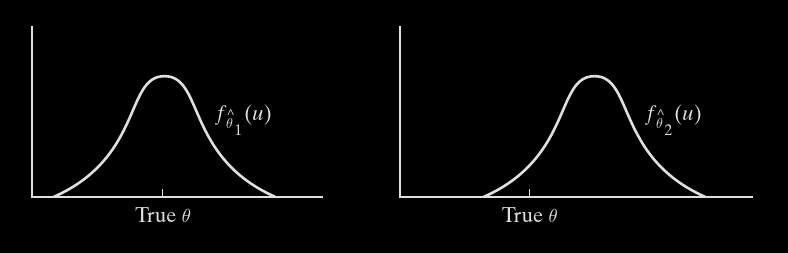
\includegraphics[scale=0.4]{Figure-5-4-2-neg.png}
\end{center}
 \vfill
 {\bf Definition 5.4.1.} Given a random sample of size $n$ whose population distribution dependes on an unknown parameter $\theta$, let $\hat{\theta}$ be an estimator of $\theta$. \\[0.5em]
 Then $\hat{\theta}$ is called {\bf unbiased} if $\E(\hat{\theta}) = \theta$; \\[0.5em]
 and $\hat{\theta}$ is called {\bf asymptotically unbiased} if $\lim_{n\rightarrow\infty}\E(\hat{\theta}) = \theta$.
\end{frame}
%-------------- end slide -------------------------------%}}}
%-------------- start slide -------------------------------%{{{ 5.49
\begin{frame}
\begin{enumerate}
% Ex 5.4.19
\item[E.g. 1.] $f_Y(y;\theta)=\frac{2y}{\theta^2}$ if $y\in [0,\theta]$.
 \begin{itemize}
  \item $\displaystyle\hat{\theta}_1=\frac{3}{2}\overline{Y}$
  \item $\displaystyle\hat{\theta}_2=Y_{max}$.
  \item $\displaystyle\hat{\theta}_3=\frac{2n+1}{2n}Y_{max}$.
 \end{itemize}
 \vfill
 \item[E.g. 2.] Let $X_1,\cdots,X_n$ be a random sample of size $n$ with the unknown parameter $\theta=\E(X)$. Show that for any constants $a_i$'s,
 \[
 \hat{\theta}=\sum_{i=1}^n a_i X_i \quad \text{is unbiased}
 \quad \Longleftrightarrow\quad
 \sum_{i=1}^n a_i=1.
 \]
\end{enumerate}
\end{frame}
%-------------- end slide -------------------------------%}}}
%-------------- start slide -------------------------------%{{{ 5.50
\begin{frame}
 \begin{enumerate}
 \item[E.g. 3.] Let $X_1,\cdots,X_n$ be a random sample of size $n$ with the unknown parameter $\sigma^2=\text{Var}(X)$.
 \begin{itemize}
  \item $\displaystyle \widehat{\sigma}^2=\frac{1}{n}\sum_{i=1}^n \left(X_i-\overline{X}\right)^2$
  \vfill
  \item $\displaystyle S^2= \text{Sample Variance} =\frac{1}{n-1}\sum_{i=1}^n \left(X_i-\overline{X}\right)^2$
  \vfill
  \item $\displaystyle S= \text{Sample Standard Deviation} =\sqrt{\frac{1}{n-1}\sum_{i=1}^n \left(X_i-\overline{X}\right)^2}$. \hfill (Biased for $\sigma$!)
 \end{itemize}
 \vfill
 \end{enumerate}
\end{frame}
%-------------- end slide -------------------------------%}}}
%-------------- start slide -------------------------------%{{{ 5.51
\begin{frame}
\begin{enumerate}
 \item[E.g. 4.] Exponential distr.: $f_Y(y;\lambda)=\lambda e^{-\lambda y}$ for $y\ge 0$. $\widehat{\lambda}=1/\overline{Y}$ is biased.\\[1em] \pause
 $n\overline{Y} = \sum_{i=1}^n Y_i\sim$ Gamma distribution$(n,\lambda)$. \pause Hence,
 \begin{align*}
 \E\left(\widehat{\lambda}\right) &= \E\left(1/\overline{Y}\right) = n\int_0^\infty \frac{1}{y} \frac{\lambda^n}{\Gamma(n)}y^{n-1}e^{-\lambda y}\ud y \\
 \pause& = \frac{n \lambda }{n-1} \int_0^\infty  \underbrace{\frac{\lambda^{n-1}}{\Gamma(n-1)}y^{(n-1)-1}e^{-\lambda y}}_{\text{pdf for Gamma distr. $(n-1,\lambda)$}} \ud y\\
 \pause &= \frac{n}{n-1}\lambda .
 \end{align*}
 Biased! But $\E(\widehat\lambda) = \frac{n}{n-1}\lambda \rightarrow \lambda$ as $n\rightarrow\infty$. (Asymptotically unbiased.)\\[1em]\pause
 Note: ~ $\widehat\lambda^*= \frac{n-1}{n \overline{Y}}$ is unbiased.
 \vfill
 \pause
 \item[E.g. 4'.] Exponential distr.: $f_Y(y;\theta)=\frac{1}{\theta} e^{-y/\theta}$ for $y\ge 0$. $\widehat{\theta}=\overline{Y}$ is unbiased. \\[1em] \pause
\[
\E\left(\widehat{\theta}\right) = \frac{1}{n} \sum_{i=1}^n \E(Y_i) = \frac{1}{n} \sum_{i=1}^n \theta = \theta.
\]
 \end{enumerate}

\end{frame}
%-------------- end slide -------------------------------%}}}
%-------------- start slide -------------------------------%{{{ 5.52
\begin{frame}{Efficiency}
 \begin{center}
 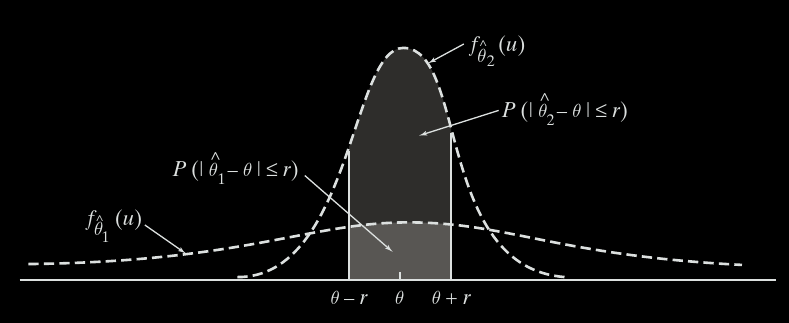
\includegraphics[scale=0.3]{Figure-5-4-3-neg.png}
\end{center}
 \vfill
 {\bf Definition 5.4.2.} Let $\widehat{\theta}_1$ and $\widehat{\theta}_2$ be two unbiased estimators for a parameter $\theta$. If $\Var(\widehat{\theta}_1)<\Var(\widehat{\theta}_2)$, then we say that $\widehat{\theta}_1$ is {\bf more efficient} than $\widehat{\theta}_2$.\\
 The {\bf relative efficiency} of $\widehat{\theta}_1$ w.r.t. $\widehat{\theta}_2$ is the ratio $\Var(\widehat{\theta}_1)/\Var(\widehat{\theta}_2)$.
\end{frame}
%-------------- end slide -------------------------------%}}}
%-------------- start slide -------------------------------%{{{ 5.53
\begin{frame}
 \begin{enumerate}
  \item[E.g. 1.] $f_Y(y;\theta)=\frac{2y}{\theta^2}$ if $y\in [0,\theta]$. Which is more efficient? Find the relative efficiency of $\widehat{\theta}_1$ w.r.t. $\widehat{\theta}_3$ .
 \begin{itemize}
  \item $\displaystyle\hat{\theta}_1=\frac{3}{2}\overline{Y}$ \\[1em]
  \item $\displaystyle\hat{\theta}_3=\frac{2n+1}{2n}Y_{max}$.
 \end{itemize}
 \vfill
 \item[E.g. 2.] Let $X_1,\cdots,X_n$ be a random sample of size $n$ with the unknown parameter $\theta=\E(X)$
	 (suppose $\sigma^2 = \Var(X)<\infty$).\\[1em]
	 \pause
	 Among all possible unbiased estimators $\hat{\theta}=\sum_{i=1}^n a_i X_i$ with $\sum_{i=1}^n a_i=1$.
	 Find the most efficient one.\\[1em]\pause
	 Sol:
 \[
 \Var(\widehat{\theta}) = \sum_{i=1}^n a_i^2 \Var(X) =\sigma^2  \sum_{i=1}^n a_i^2
 \ge \sigma^2 \frac{1}{n} \left(\sum_{i=1}^n a_i\right)^2 = \frac{1}{n} \sigma^2,
 \]
 \[
 \text{with equality iff $a_1=\cdots=a_n=1/n$.}
 \]
 Hence, the most efficient one is the sample mean $\widehat\theta= \overline{X}$.
 \myEnd
 \end{enumerate}

\end{frame}
%-------------- end slide -------------------------------%}}}
